% ============================================================
%  Curriculum Vitae — Rocélio da Silva
%  EN — Formal Executive: White, Black & Navy
% ============================================================
\documentclass[10pt,a4paper]{article}

\usepackage[utf8]{inputenc}
\usepackage[T1]{fontenc}
\usepackage[margin=0pt]{geometry}
\usepackage{array,tabularx}
\usepackage{enumitem}
\usepackage{hyperref}
\usepackage{xcolor}
\usepackage{graphicx}
\usepackage{tikz}
\usepackage{setspace}
\usepackage{parskip}
\usepackage{amssymb}

\usetikzlibrary{calc}

% ============================================================
%  COLOURS — Formal white document
% ============================================================
\definecolor{navy}{HTML}{1A3A5C}
\definecolor{navylt}{HTML}{2E5F8A}
\definecolor{goldrule}{HTML}{C8A84B}
\definecolor{bodytext}{HTML}{1A1A1A}
\definecolor{mutedtext}{HTML}{555555}
\definecolor{sidetext}{HTML}{EEF4FA}
\definecolor{sidebg}{HTML}{1A3A5C}

% ============================================================
%  GLOBAL
% ============================================================
\color{bodytext}
\pagestyle{empty}
\setlength{\parindent}{0pt}
\setlength{\parskip}{2pt}

\hypersetup{colorlinks=true, urlcolor=navylt, linkcolor=navylt}

% ============================================================
%  SIDEBAR SECTION
% ============================================================
\newcommand{\sideSection}[1]{%
  \vspace{5pt}%
  {\bfseries\color{sidetext}\small\MakeUppercase{#1}}%
  \par\vspace{1pt}%
  {\color{goldrule}\rule{\linewidth}{0.55pt}}%
  \par\vspace{2pt}%
}

% ============================================================
%  MAIN SECTION
% ============================================================
\newcommand{\mainSection}[1]{%
  \vspace{4pt}%
  {\bfseries\color{navy}\large\MakeUppercase{#1}}%
  \par\vspace{0pt}%
  {\color{navy}\rule{\linewidth}{1.0pt}}%
  \par\vspace{2pt}%
}

% ============================================================
%  EXPERIENCE ENTRY
% ============================================================
\newcommand{\expEntry}[3]{%
  {\bfseries\color{navy}\normalsize #1}\par\vspace{1pt}%
  {\color{mutedtext}\small #2 \hfill \textit{\color{navylt}#3}}\par\vspace{1pt}%
}

% ============================================================
%  LISTS
% ============================================================
\setlist[itemize]{
  itemsep=0pt,
  topsep=0pt,
  leftmargin=1.3em,
  label={\color{navylt}\small$\bullet$}
}

\begin{document}

% ============================================================
%  SIDEBAR BACKGROUND
% ============================================================
\noindent
\begin{tikzpicture}[remember picture, overlay]
  \fill[sidebg]
    (current page.north west)
    rectangle
    ([xshift=0.295\paperwidth] current page.south west);
  \draw[goldrule, line width=1.0pt]
    ([xshift=0.295\paperwidth] current page.north west)
    -- ([xshift=0.295\paperwidth] current page.south west);
\end{tikzpicture}

% ============================================================
%  LEFT SIDEBAR
% ============================================================
\noindent
\begin{minipage}[t]{0.283\paperwidth}
  \color{sidetext}
  \setlength{\parskip}{3pt}
  \hspace*{10pt}%
  \begin{minipage}[t]{\dimexpr\linewidth-18pt}

    \vspace{5pt}
    \begin{center}
      \IfFileExists{photo.png}{%
        \begin{tikzpicture}
          \clip (0,0) circle (0.72in);
          \node[inner sep=0pt] at (0,0)
            {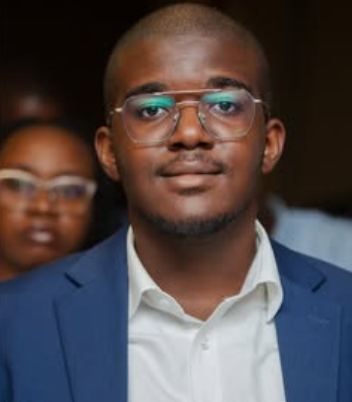
\includegraphics[width=1.44in,height=1.44in,keepaspectratio]{photo.png}};
          \draw[white, line width=2pt] (0,0) circle (0.72in);
        \end{tikzpicture}%
      }{%
        
\begin{tikzpicture}
          \fill[white] (0,0) circle (0.72in);
          \draw[goldrule, line width=1.6pt] (0,0) circle (0.72in);
          \node[font=\bfseries\LARGE, text=navy] at (0,0) {RS};
        \end{tikzpicture}%
      }
      \par\vspace{2pt}
      {\large\bfseries\color{white} Rocélio da Silva}\par\vspace{2pt}
      {\small\color{sidetext!80} Offshore \& Upstream Engineering}\par\vspace{2pt}
      {\color{goldrule}\rule{0.70\linewidth}{0.5pt}}
    \end{center}

    \sideSection{Contact}
    {\small
      \textbf{\color{white}Tel\,} \color{sidetext}+244 924 010 222\par\vspace{2pt}
      \textbf{\color{white}Email\,} \href{mailto:rocelioinc@gmail.com}{\color{goldrule!80}rocelioinc@gmail.com}\par\vspace{2pt}
      \textbf{\color{white}Location\,} \color{sidetext}Benfica, Luanda\par
    }

    \sideSection{Education}
    {\small
      \textbf{\color{white}ISPTEC}\par
      \color{sidetext}B.Sc.\ Petroleum Engineering\par
      \textit{\color{goldrule!80}2022 -- Present $\cdot$ 3rd Year}\par\vspace{2pt}
      \textbf{\color{white}CEPI}\par
      \color{sidetext}Secondary School Diploma\par
      \textit{\color{goldrule!80}2020 -- 2022}\par
    }

    \sideSection{Languages}
    {\small
      \begin{tabular}{@{}l@{\hspace{6pt}}r@{}}
        \textbf{\color{white}Portuguese} & \color{sidetext}Native \\[3pt]
        \textbf{\color{white}English}    & \color{goldrule!90}TOEFL 99 \\
      \end{tabular}
    }

    \sideSection{Technical Skills}
    {\small
      \begin{itemize}[leftmargin=1em,
                      label={\color{goldrule}\tiny$\blacktriangleright$},
                      itemsep=0pt, topsep=1pt]
        \item \color{sidetext}Python -- Pandas, Matplotlib
        \item \color{sidetext}Z-Factor Calc.\ (Pitzer, Papay)
        \item \color{sidetext}EOR Method Selection
        \item \color{sidetext}Reservoir \& Well Eng.
        \item \color{sidetext}Offshore Drilling Fluids
        \item \color{sidetext}GIS $\cdot$ Blender 3-D
        \item \color{sidetext}C,\; HTML / CSS
      \end{itemize}
    }

    \sideSection{Leadership}
    {\small
      \begin{itemize}[leftmargin=1em,
                      label={\color{goldrule}\tiny$\blacktriangleright$},
                      itemsep=0pt, topsep=1pt]
        \item \color{sidetext}Membership Chairperson
        \item \color{sidetext}Event Management
        \item \color{sidetext}Technical Communication
        \item \color{sidetext}Teamwork
      \end{itemize}
    }

    \sideSection{Affiliations}
    {\small
      \textbf{\color{white}SPE} \color{sidetext}-- Soc.\ of Petroleum Engineers\par
      \textit{\color{goldrule!80}Student Member}\par\vspace{2pt}
      \textbf{\color{white}MIT Global Classroom}\par
      \textit{\color{goldrule!80}Participant, 2025}\par
    }

    \vspace{4pt}
    \begin{center}
      {\color{goldrule}\rule{0.55\linewidth}{0.4pt}}\par\vspace{2pt}
      {\color{sidetext!60}\small\itshape References upon request}
    \end{center}

  \end{minipage}
\end{minipage}%
%
% ============================================================
%  RIGHT — MAIN CONTENT  (white background, dark text)
% ============================================================
\hspace*{10pt}%
\begin{minipage}[t]{\dimexpr 0.705\paperwidth - 26pt}
  \color{bodytext}
  \setlength{\parskip}{2pt}
  \setstretch{1.02}

  \vspace{5pt}

  % ---- NAME HEADER ----
  {\huge\bfseries\color{navy} ROCÉLIO DA SILVA}\par
  \vspace{2pt}
  {\normalsize\color{mutedtext}
    Offshore \& Upstream Engineering
    $\cdot$ SPE Member
    $\cdot$ Luanda, Angola
  }\par
  \vspace{2pt}
  {\color{navy}\rule{\linewidth}{1.2pt}}\par
  \vspace{1pt}
  {\color{goldrule}\rule{\linewidth}{0.4pt}}

  % ---- PROFILE ----
  \mainSection{Profile}
  \setstretch{1.02}
  3rd-year Petroleum Engineering student at ISPTEC with a strong drive for
  \textbf{offshore} operations and technical software development for the oil \& gas
  industry. ISPTEC team leader at PetroChamp, SPE Student Chapter Membership
  Chairperson and MIT Global Classroom participant (2025). Builds Python tools for
  reservoir engineering (Z-factor, EOR selection). Fluent in English (TOEFL~99)
  and committed to technical excellence in emerging markets.
  \setstretch{1.02}

  % ---- PROFESSIONAL EXPERIENCE ----
  \mainSection{Professional Experience}

  \expEntry{Membership Chairperson -- SPE Student Chapter}%
           {ISPTEC / Society of Petroleum Engineers}%
           {2026 -- Present}
  \begin{itemize}
    \item Leads member recruitment, engagement and retention.
    \item Coordinates technical seminars and fosters industry--academia networking.
  \end{itemize}

  \vspace{3pt}
  \expEntry{Secretary of Academic Affairs}%
           {AEISPTEC -- ISPTEC Student Association}%
           {2025}
  \begin{itemize}
    \item Coordinated academic events and departmental activities.
    \item Managed student communications and academic documentation.
    \item Acted as liaison between academic leadership and the student body.
  \end{itemize}

  % ---- KEY PROJECTS ----
  \mainSection{Key Projects}

  {\small\bfseries\color{navy}Community Solar Feasibility Study -- MIT-ISPTEC (2025)}\par
  {\footnotesize\color{mutedtext}MIT Global Classroom $\cdot$ Angola Energy Access Initiative}
  \begin{itemize}
    \item Optimal site selection via GIS analysis and energy demand modelling.
    \item Presented findings to international stakeholders and ISPTEC leadership.
    \item Direct impact on energy access strategy for underserved communities across Angola.
  \end{itemize}

  \vspace{3pt}
  {\small\bfseries\color{navy}Z-Factor \& EOR Decision Tool -- Python (2024--2025)}\par
  {\footnotesize\color{mutedtext}Software Engineering $\cdot$ ISPTEC}
  \begin{itemize}
    \item Python Z-factor calculator (Pitzer--Curl, Papay) for reservoir conditions.
    \item EOR method selection module: multi-criteria analysis (WAG, polymers,
          CO\textsubscript{2} flooding).
    \item Interactive CLI; CSV export and Matplotlib charts.
  \end{itemize}

  % ---- ACHIEVEMENTS ----
  \mainSection{Achievements \& Recognition}

  \renewcommand{\arraystretch}{1.40}
  \begin{tabular}{@{} p{0.06\linewidth} p{0.88\linewidth} @{}}
    {\footnotesize\bfseries\color{navy}2025} &
      \textbf{PetroChamp -- ISPTEC Team Leader:} Led the ISPTEC team in the
      PetroChamp technical competition, demonstrating academic excellence and
      leadership under pressure.\\
    {\footnotesize\bfseries\color{navy}2025} &
      \textbf{Host \& Speaker} -- ISPTEC Geosciences Academic Week;
      coordinated multinational speakers.\\
    {\footnotesize\bfseries\color{navy}2025} &
      \textbf{MIT Global Classroom} -- Community Solar Energy Access; study
      presented to international collaborators.\\
    {\footnotesize\bfseries\color{navy}2022} &
      \textbf{TOEFL 99/120} -- Advanced English proficiency enabling SPE
      and MIT international collaborations.\\
  \end{tabular}
  \renewcommand{\arraystretch}{1}

  % ---- CAREER OBJECTIVES ----
  \mainSection{Career Objectives}
  \setstretch{1.02}
  Seeking a position in \textbf{offshore} or upstream petroleum engineering where I can
  combine reservoir engineering knowledge, technical software development in Python
  and team leadership to contribute to efficient, sustainable operations in Angola
  and sub-Saharan Africa.
  \setstretch{1.02}

  \vspace{6pt}
  {\color{navy}\rule{\linewidth}{0.8pt}}\par
  \vspace{1pt}
  {\color{goldrule}\rule{\linewidth}{0.4pt}}\par
  \vspace{3pt}
  {\footnotesize\color{mutedtext}\itshape
    Petroleum Engineering $\cdot$ Angola $\cdot$ 2025}

\end{minipage}

\end{document}
